%%%%%%%%%%%% PREAMBLE %%%%%%%%%%%%%%%%%%%%%

% Initiate document
% -----------------
\documentclass[11pt,a4paper]{article}

% Document codification and language
\usepackage[utf8]{inputenc} % Codificação do documento (conversão automática dos acentos)
\usepackage[T1]{fontenc}
\usepackage[USenglish]{babel}

% Set up geometry of the document
\usepackage{geometry}
\geometry{a4paper,tmargin=2.54cm,bmargin=2.54cm,lmargin=2.54cm,rmargin=2.54cm}

% Load packages
% -------------
\usepackage[centertags]{amsmath}
\usepackage{amssymb}
\usepackage{amsthm}
\usepackage{amsfonts}
\usepackage{latexsym}
\usepackage{graphicx}

\usepackage{epstopdf} %converting to PDF
\usepackage{polynom}
\usepackage{verbatim}
\usepackage{rotating}

\usepackage{setspace}
\usepackage[section]{placeins}
\usepackage[justification=centering]{caption}
\usepackage{tabularx}
\usepackage{booktabs}
\usepackage{multirow}

\def\sym#1{\ifmmode^{#1}\else\(^{#1}\)\fi} %for \sym{*}

\usepackage{array}
\newcolumntype{C}{>{\centering\arraybackslash}m{2cm}}
\newcolumntype{D}{>{\centering\arraybackslash}m{1.81cm}}

\usepackage{color}
\setcounter{tocdepth}{4}
\usepackage{adjustbox}
\usepackage{pgfplots}
\usepackage{graphicx}
\usepackage{afterpage}
\usepackage{lscape}
%\usepackage{subfigure} is an obsolete package
\usepackage{subcaption} %is the new one
\usepackage[bottom]{footmisc}
\usepackage{longtable}
\usepackage{ragged2e}
\usepackage{pdflscape}
\usepackage{titlesec}

% HYPERLINKS
\usepackage[hyphens]{url}
\usepackage[backref]{hyperref}
\hypersetup{colorlinks=true,
	linkcolor=black,
	urlcolor=blue,
	citecolor=gray}

\renewcommand\backrefxxx[3]{%
	\hyperlink{page.#1}{\textcolor{red}{$\uparrow$#1}}%
}

\usepackage{scalerel,stackengine}
\stackMath
\newcommand\reallywidehat[1]{%
	\savestack{\tmpbox}{\stretchto{%
			\scaleto{%
				\scalerel*[\widthof{\ensuremath{#1}}]{\kern-.6pt\bigwedge\kern-.6pt}%
				{\rule[-\textheight/2]{1ex}{\textheight}}%WIDTH-LIMITED BIG WEDGE
			}{\textheight}% 
		}{0.5ex}}%
	\stackon[1pt]{#1}{\tmpbox}%
}

\usepackage[round]{natbib}
\bibliographystyle{ecta}

\usepackage{pdfpages}

\renewcommand{\thepage}{\roman{page}} % Roman numerals for page counter

\pgfplotsset{compat=1.14}
\begin{document}
	
	% Title page
	% ----------
	
	\font\myfont=cmr12 at 19pt
	\title{\myfont{Online Appendix for ``Supporting Teacher Autonomy to Improve Education Outcomes: Experimental Evidence from Brazil''}}
	
	\newcommand*\samethanks[1][\value{footnote}]{\footnotemark[#1]}
	
	\author{%
		Caio Piza\thanks{Development Impact Evaluation (DIME), The World Bank, 1818 H Street NW, Washington, DC 20433, United States.}%
		\and Astrid Zwager\samethanks[2]%
		\and Matteo Ruzzante\samethanks[2]%
		\and Rafael Dantas\samethanks[2]%
		\and Andre Loureiro\thanks{Education Global Practice, The World Bank.}
	}
	
	\date{}
	
	\maketitle
	
	% Contents and lists
	\vspace{1cm}
	\listoffigures
	\listoftables
	
	
	\newpage
	\sloppy
	
	% Set up paragraph
	\doublespacing
	
	\setlength\parskip{1em}
	\setlength\parindent{0pt}
	
	\titlespacing{\section}{0pt}{0.5\parskip}{*-0.75}
	\titlespacing{\subsection}{0pt}{0.5\parskip}{*-0.75}
	\titlespacing{\subsubsection}{0pt}{0.5\parskip}{*-0.75}
	
	%%%%%%%%%%%%%%%%%%%%%%%%%%%%%%%%%%%%%%%%%%%%%%%%%%%%%%%%%%%%%%%%%%%%%%%%%%%%%%%
	
	% Attach DIME Analytics 
	\pgfplotsset{compat=1.15}
	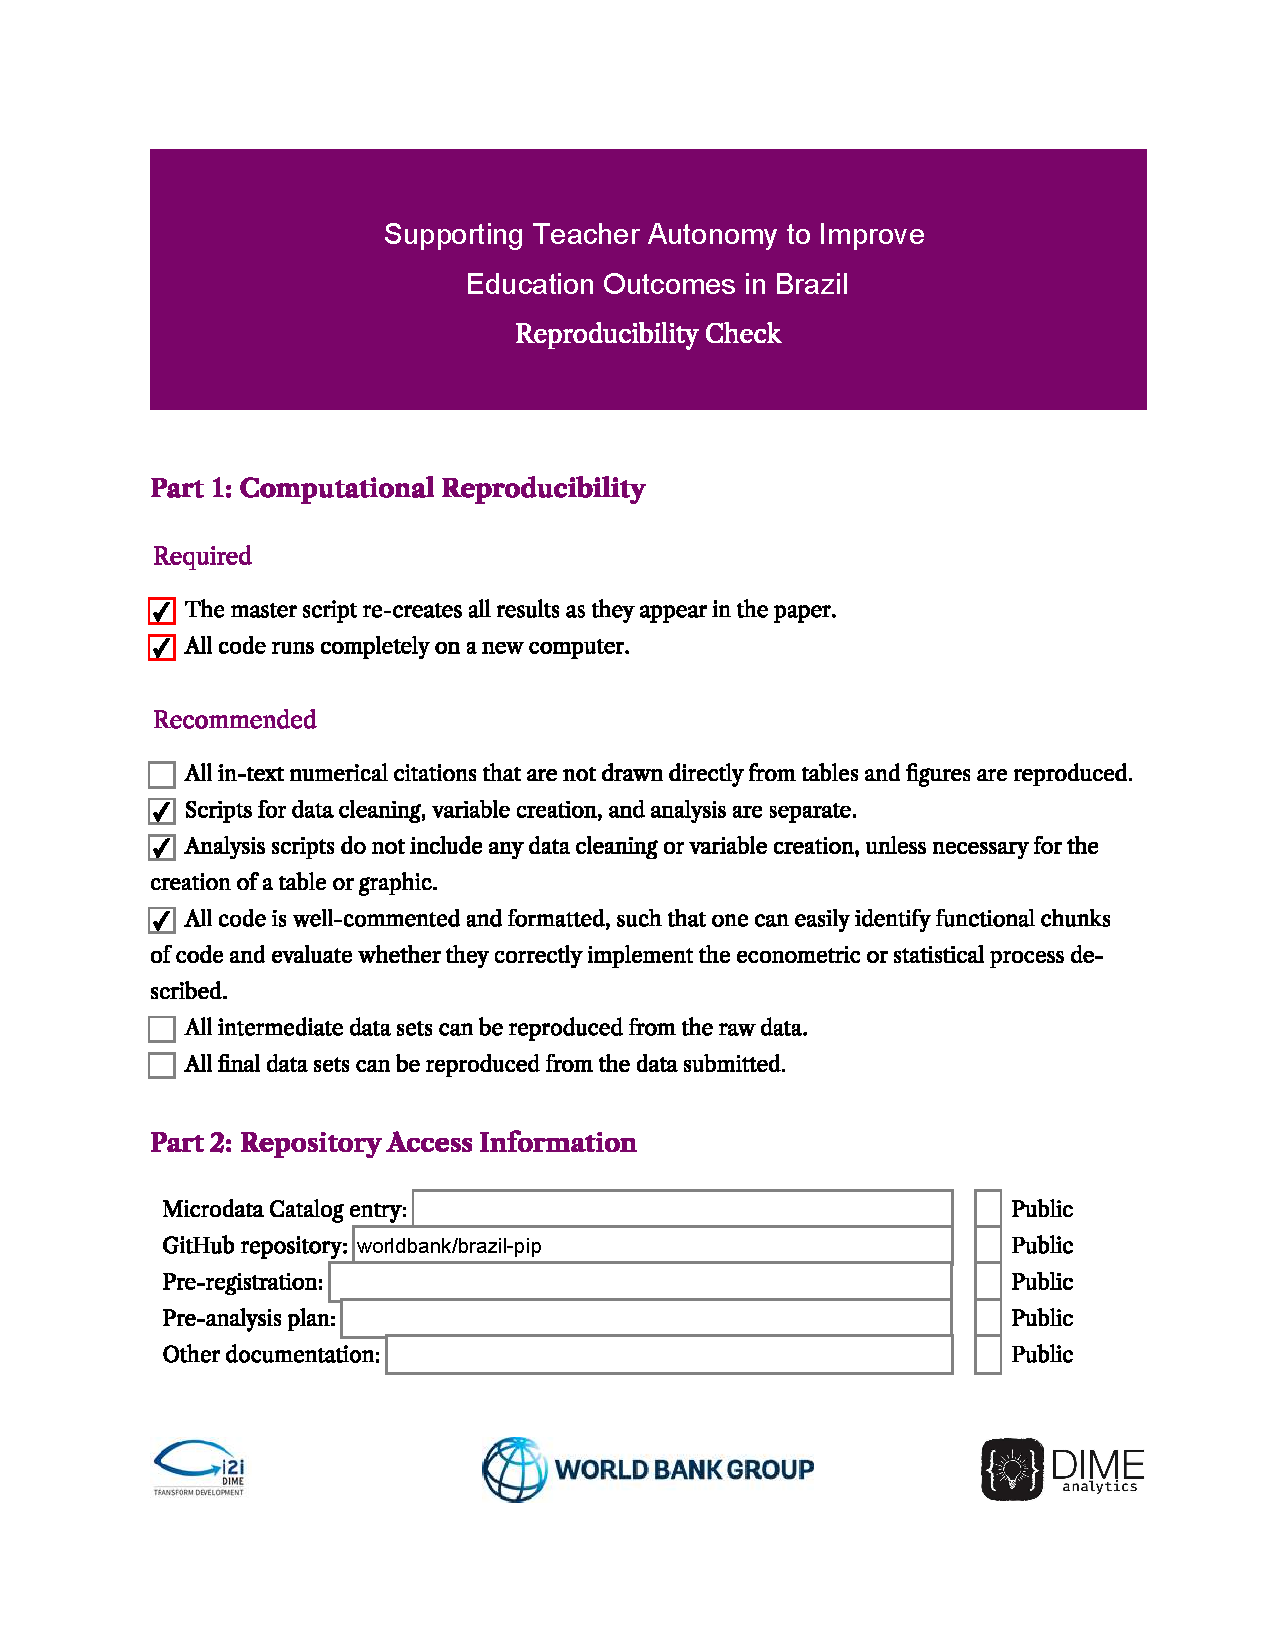
\includepdf[pages=-, fitpaper=true]{ReproducibilityCheck}
	
	\newpage
	\renewcommand{\thetable}{C\arabic{table}}
	\renewcommand{\thefigure}{C\arabic{figure}}
	
	\clearpage
	\null
	\vfill
	\begin{figure}[ht!]
		\centering
		\caption{Quantile Treatment Effects in 6\textsuperscript{th} Grade -- By Subject}
		\captionsetup[subfigure]{justification=centering}
		\label{fig:qreg_bySubject_grade6}
		
		\begin{subfigure}{0.5\textwidth}
			\centering
			\caption{Math}
			\label{fig:qreg_MT_grade6}
			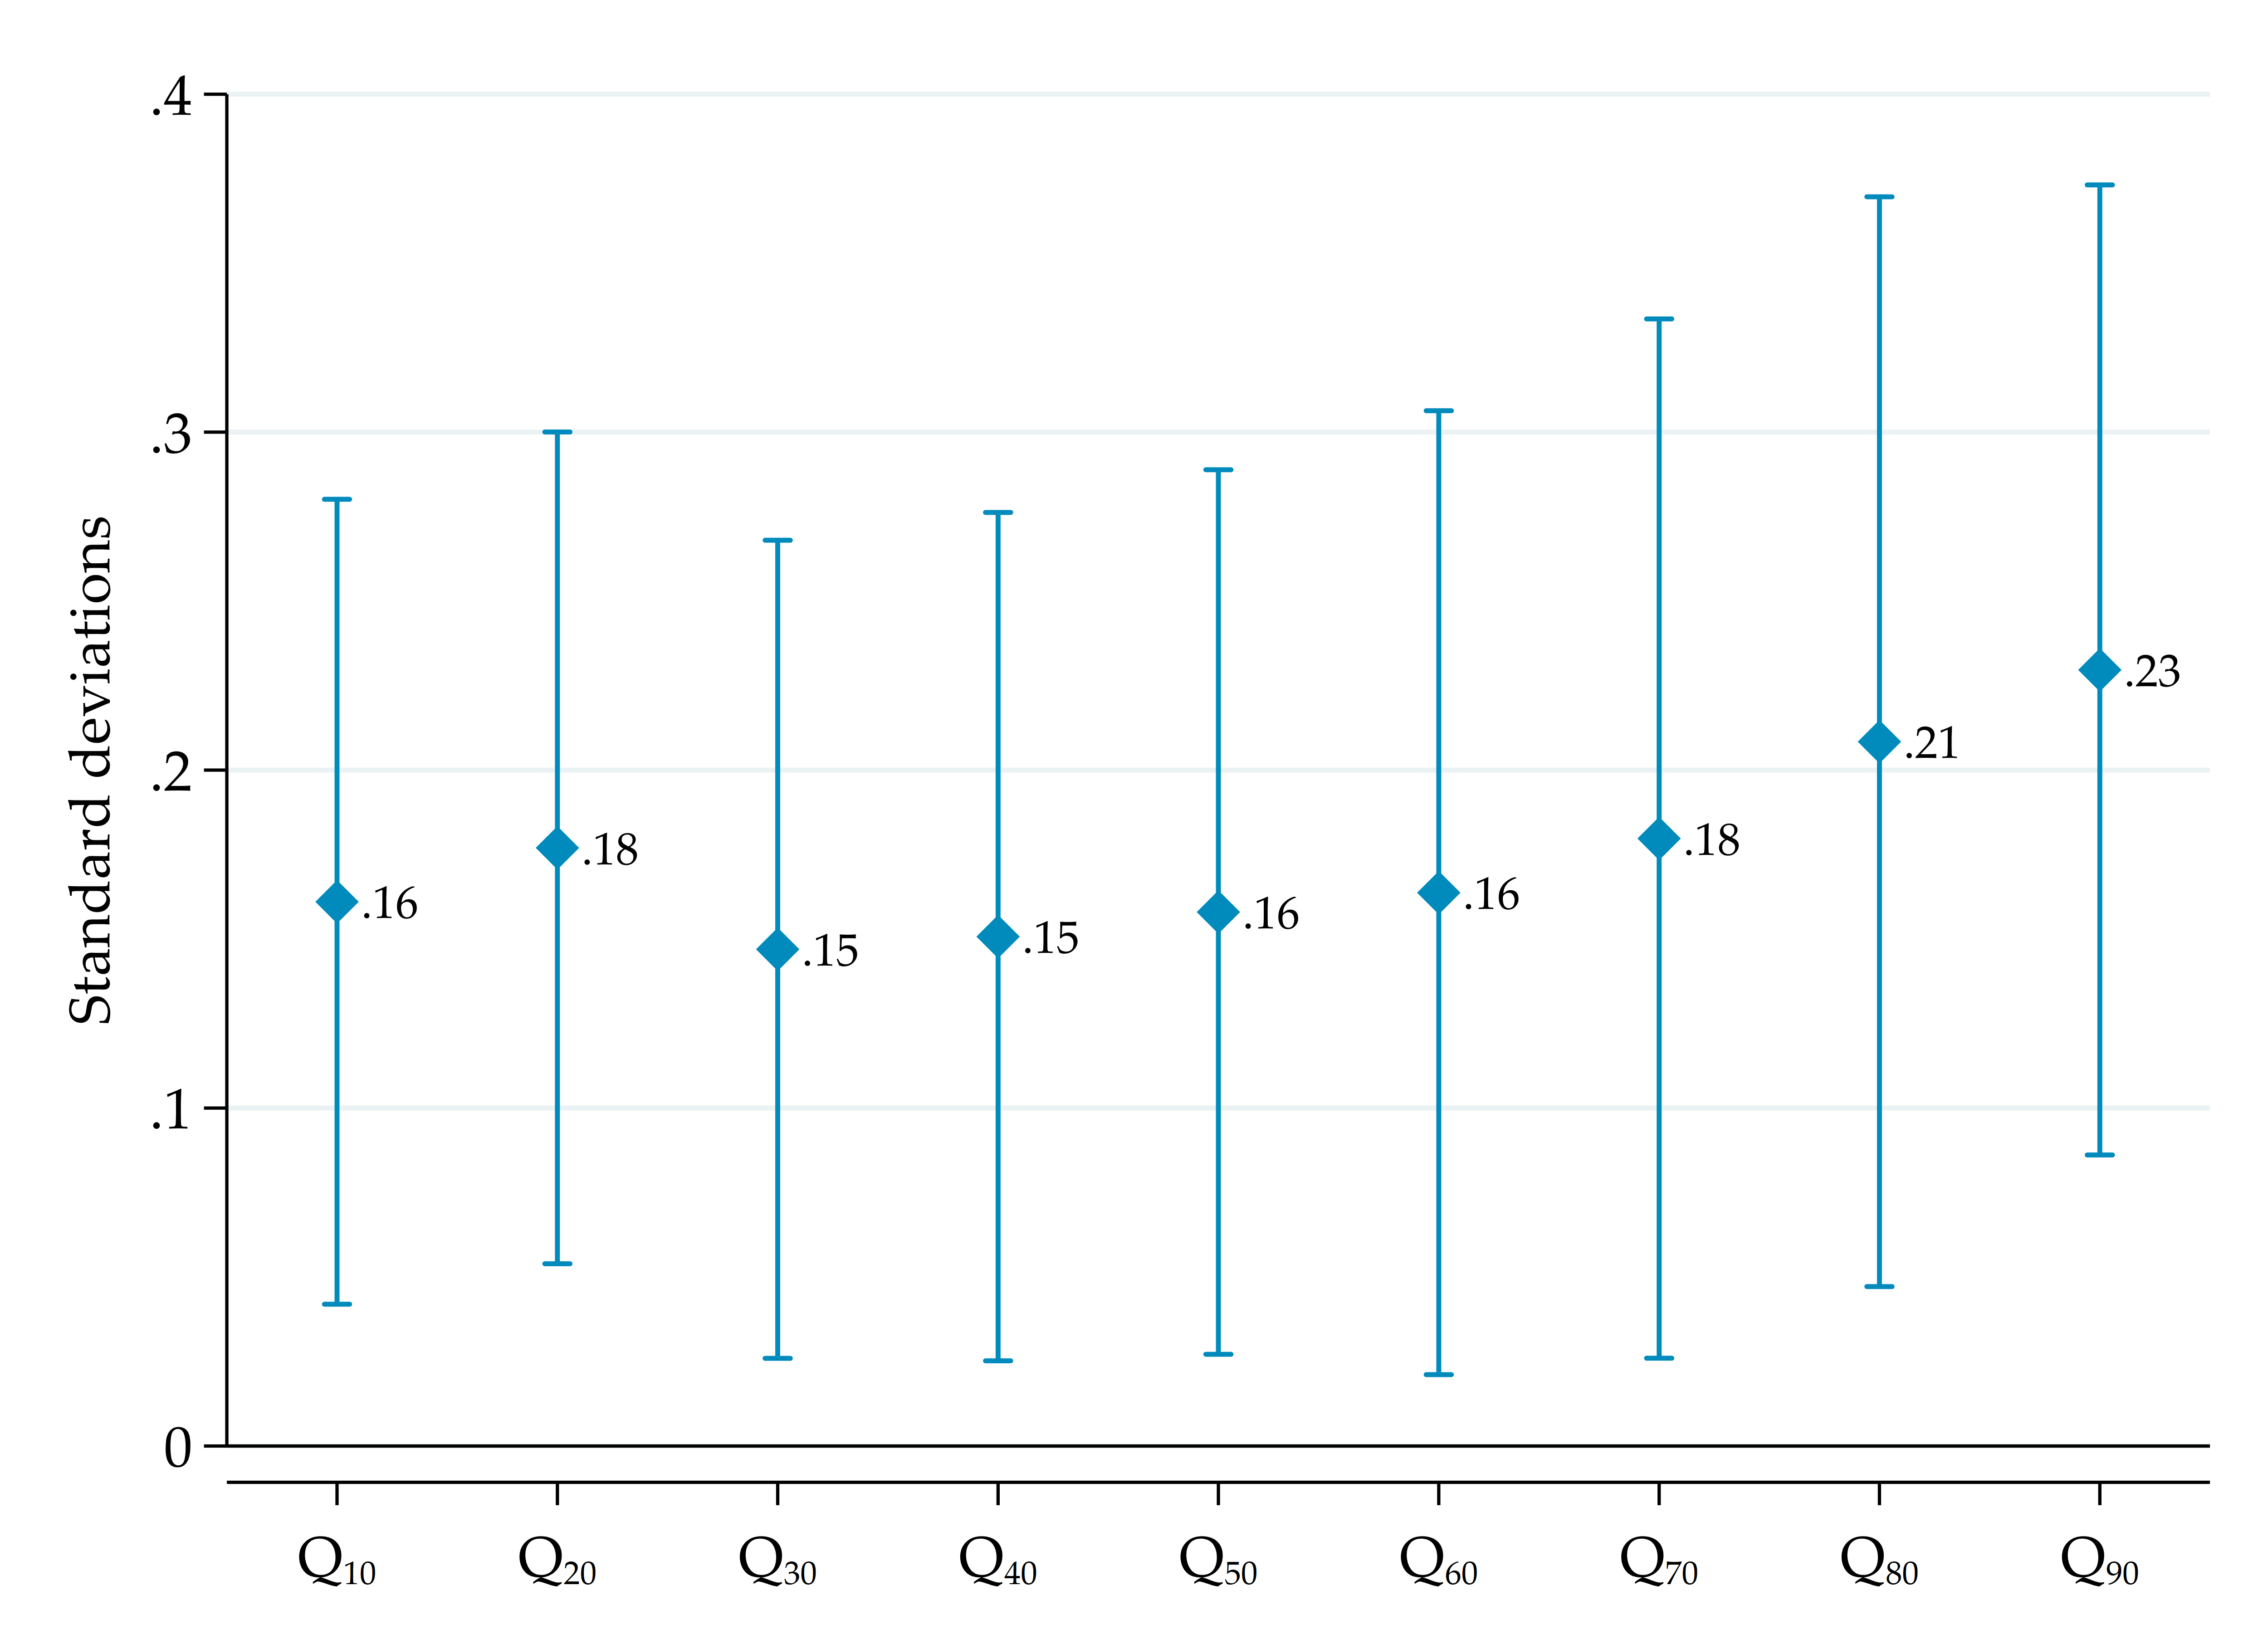
\includegraphics[width=8cm]{DataWork/Output/Figures/figC1a-qreg_MT_grade6.png}
		\end{subfigure}%
		\begin{subfigure}{0.5\textwidth}
			\centering
			\caption{Portuguese}
			\label{qreg_LT_grade6}
			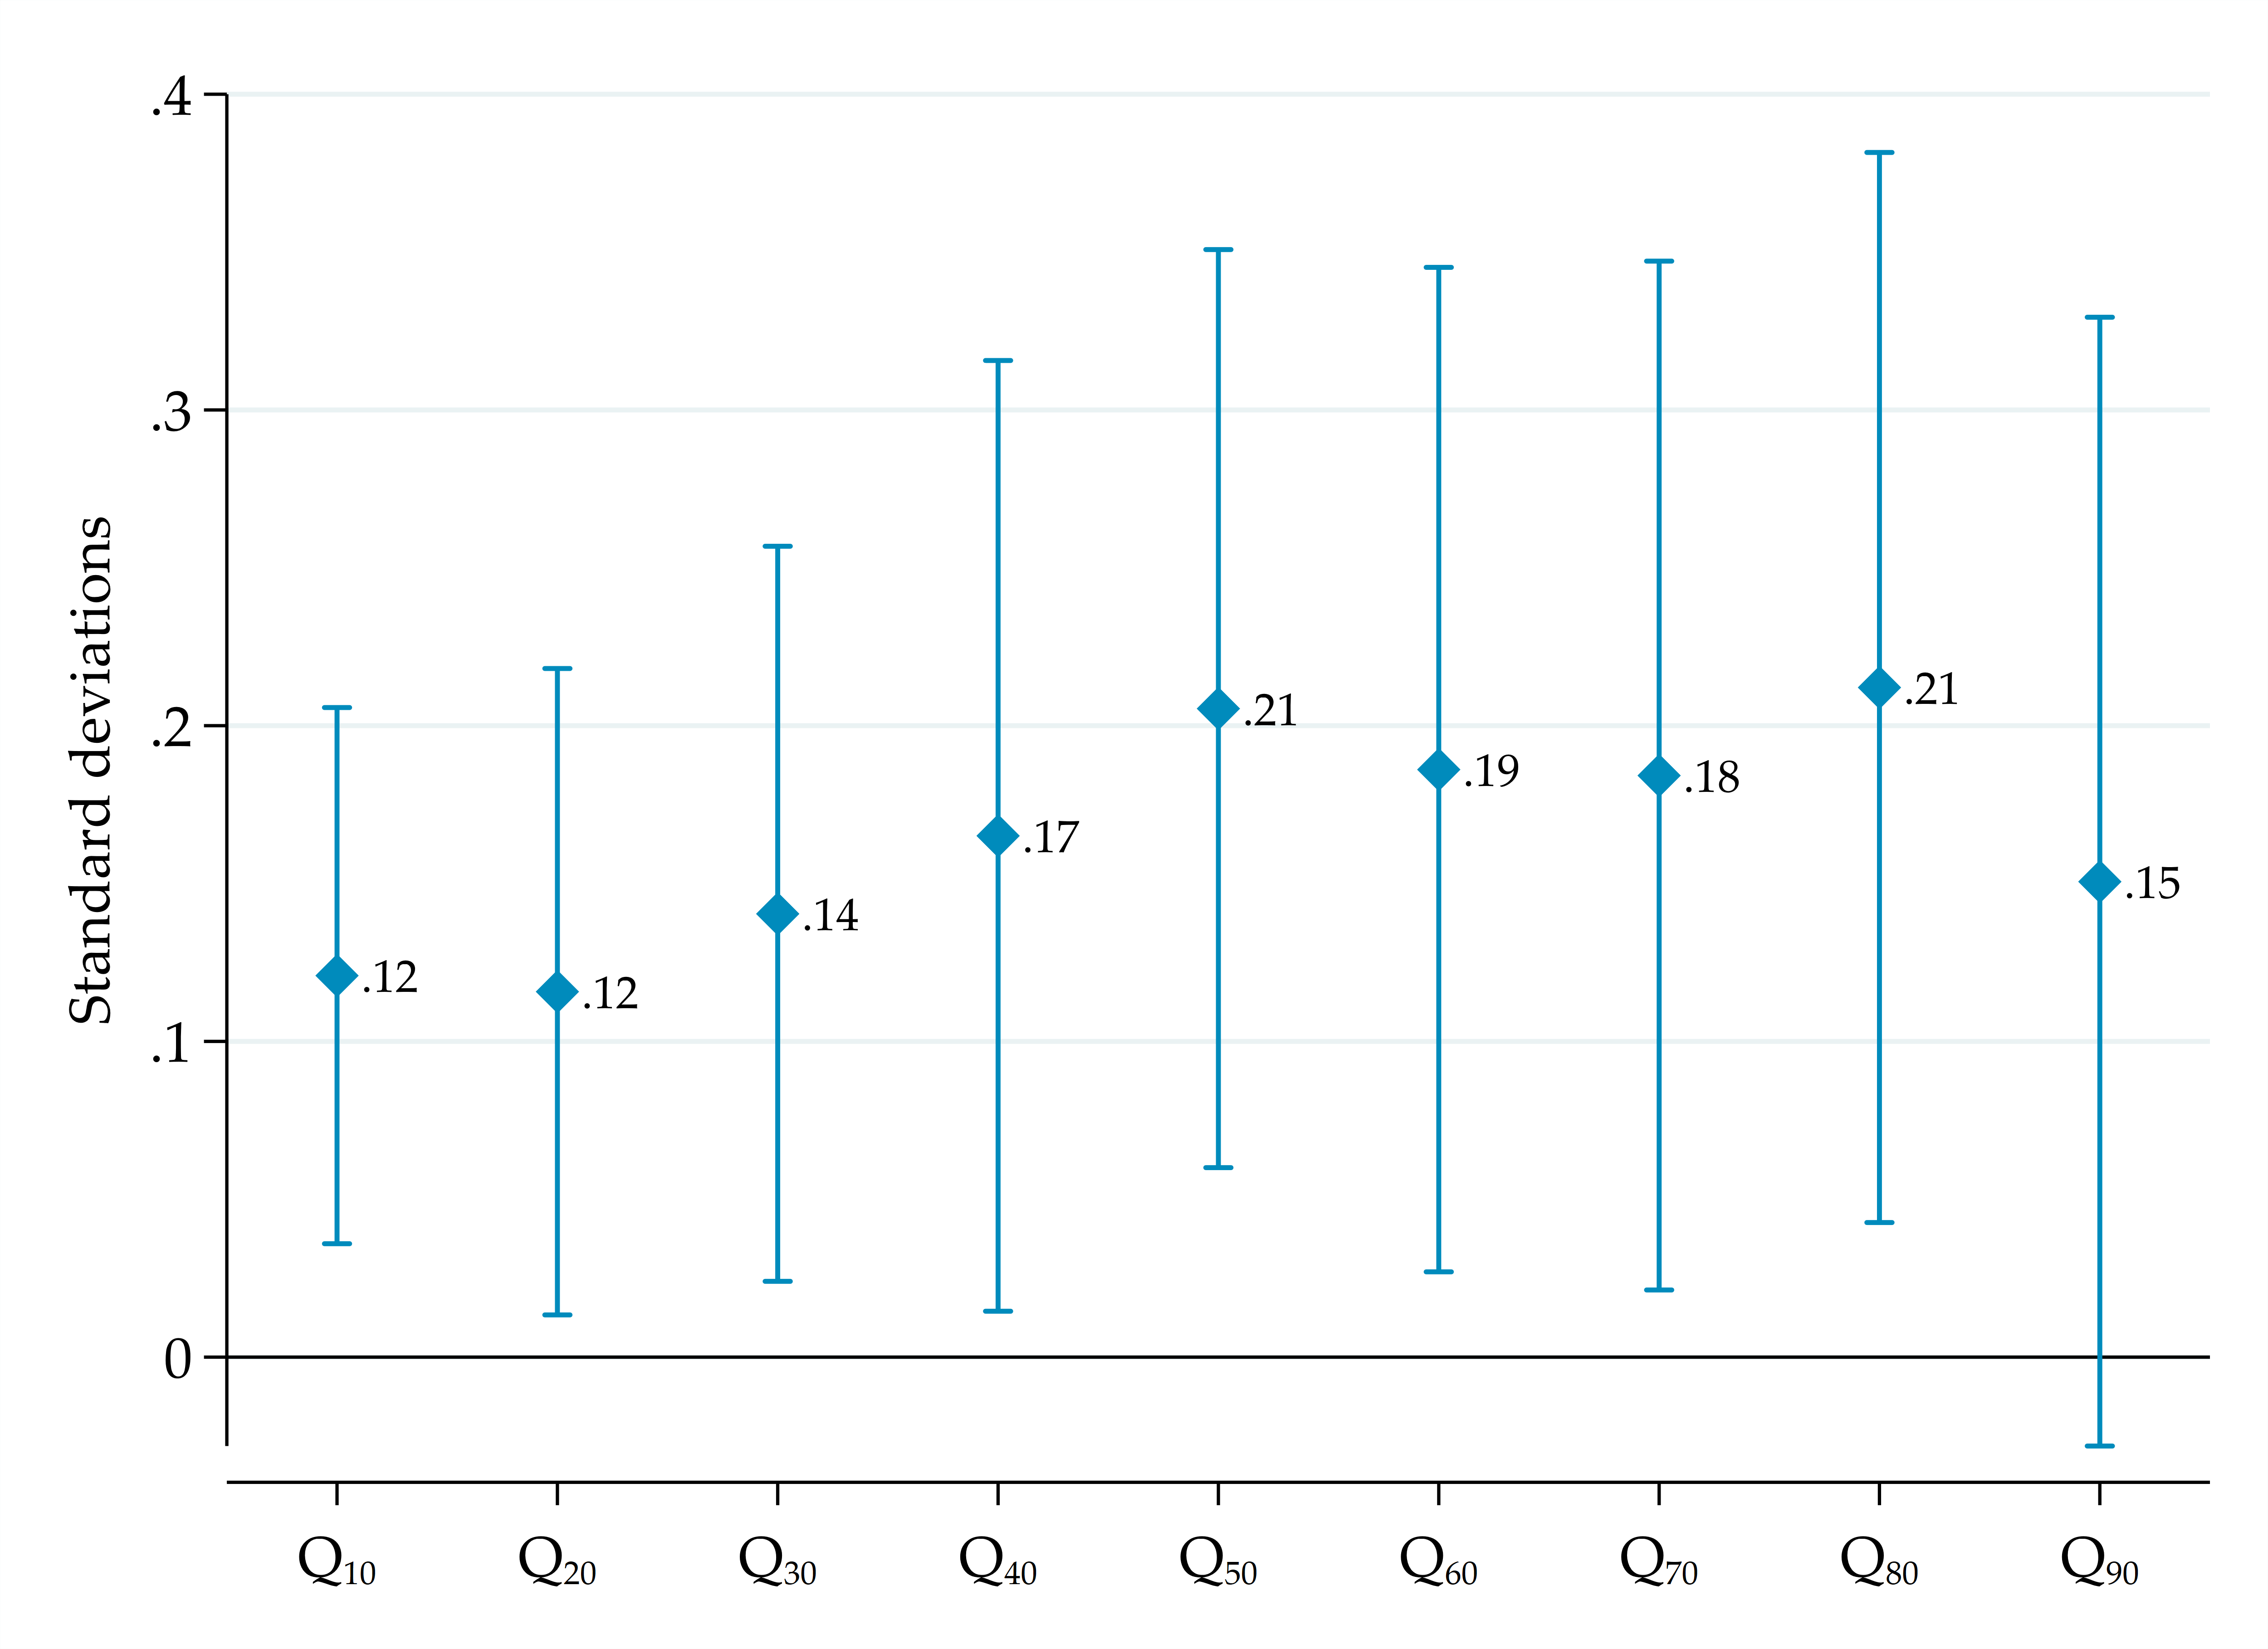
\includegraphics[width=8cm]{DataWork/Output/Figures/figC1b-qreg_LT_grade6}
		\end{subfigure} 
		
		\vspace{1em}
		
		\begin{subfigure}{0.5\textwidth}
			\centering
			\caption{Human Sciences}
			\label{fig:qreg_CH_grade6}
			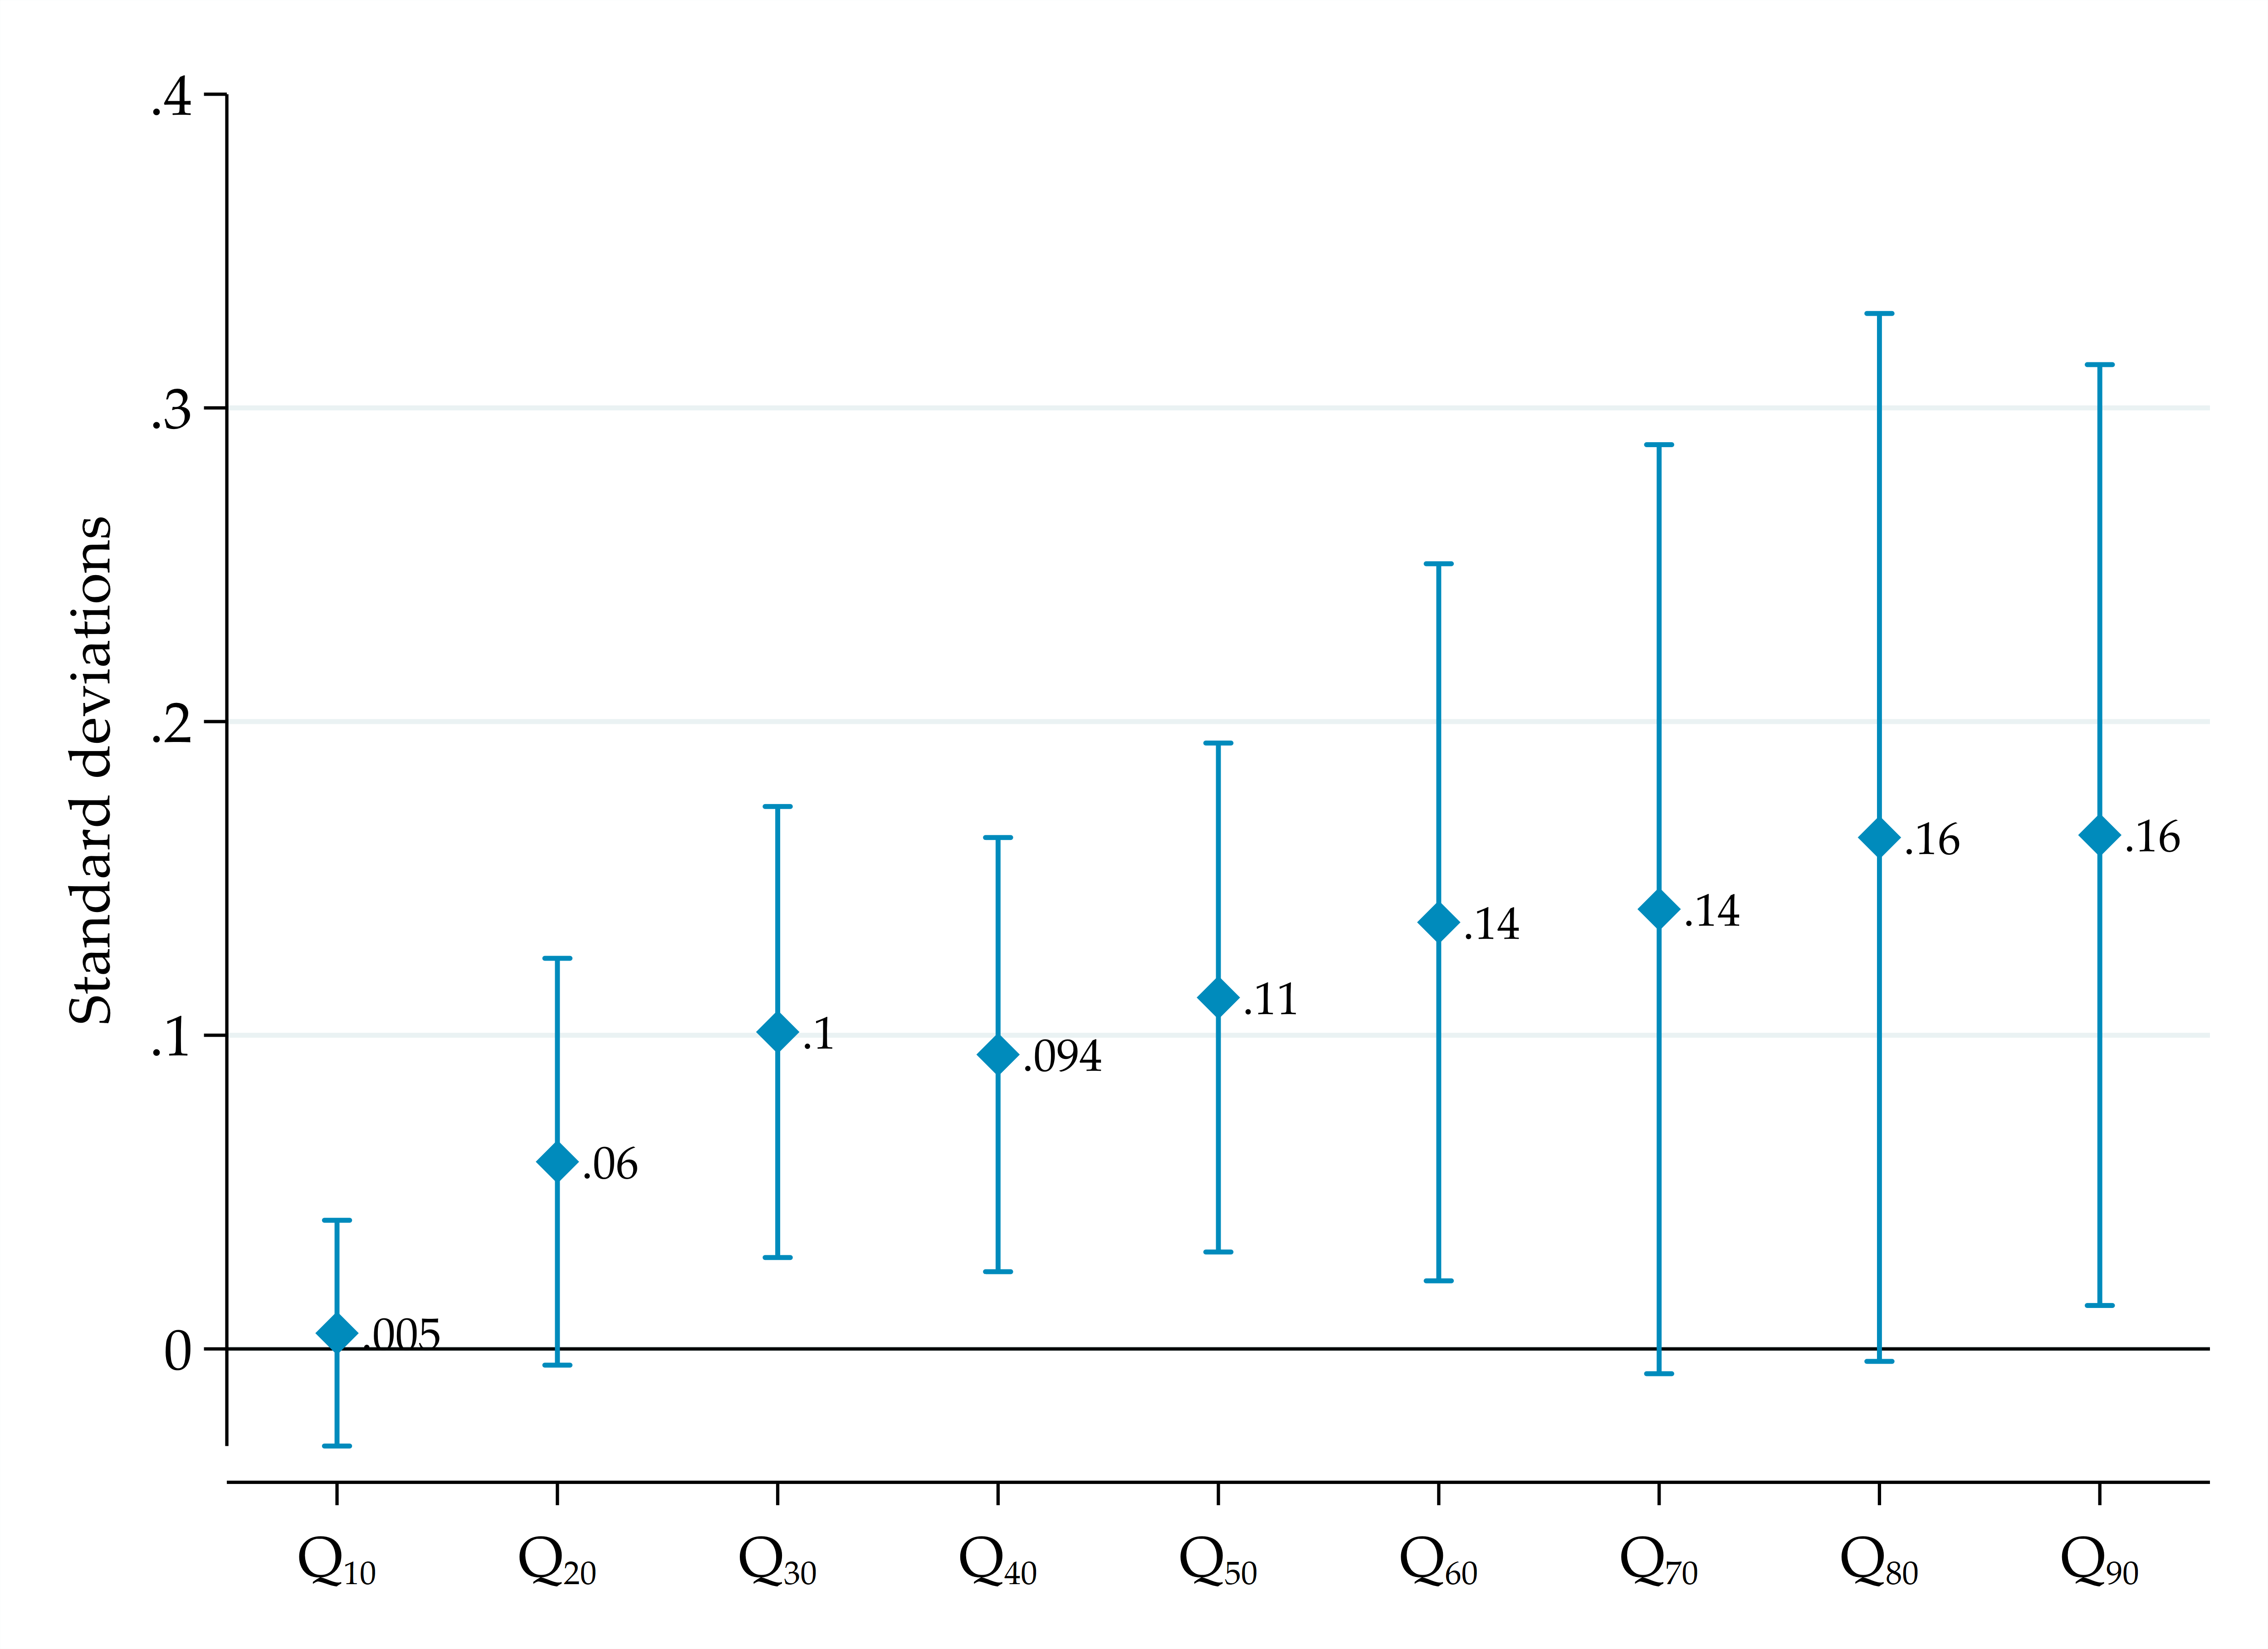
\includegraphics[width=8cm]{DataWork/Output/Figures/figC1c-qreg_CH_grade6.png}
		\end{subfigure}%
		\begin{subfigure}{0.5\textwidth}
			\centering
			\caption{Natural Sciences}
			\label{fig:qreg_CN_grade6}
			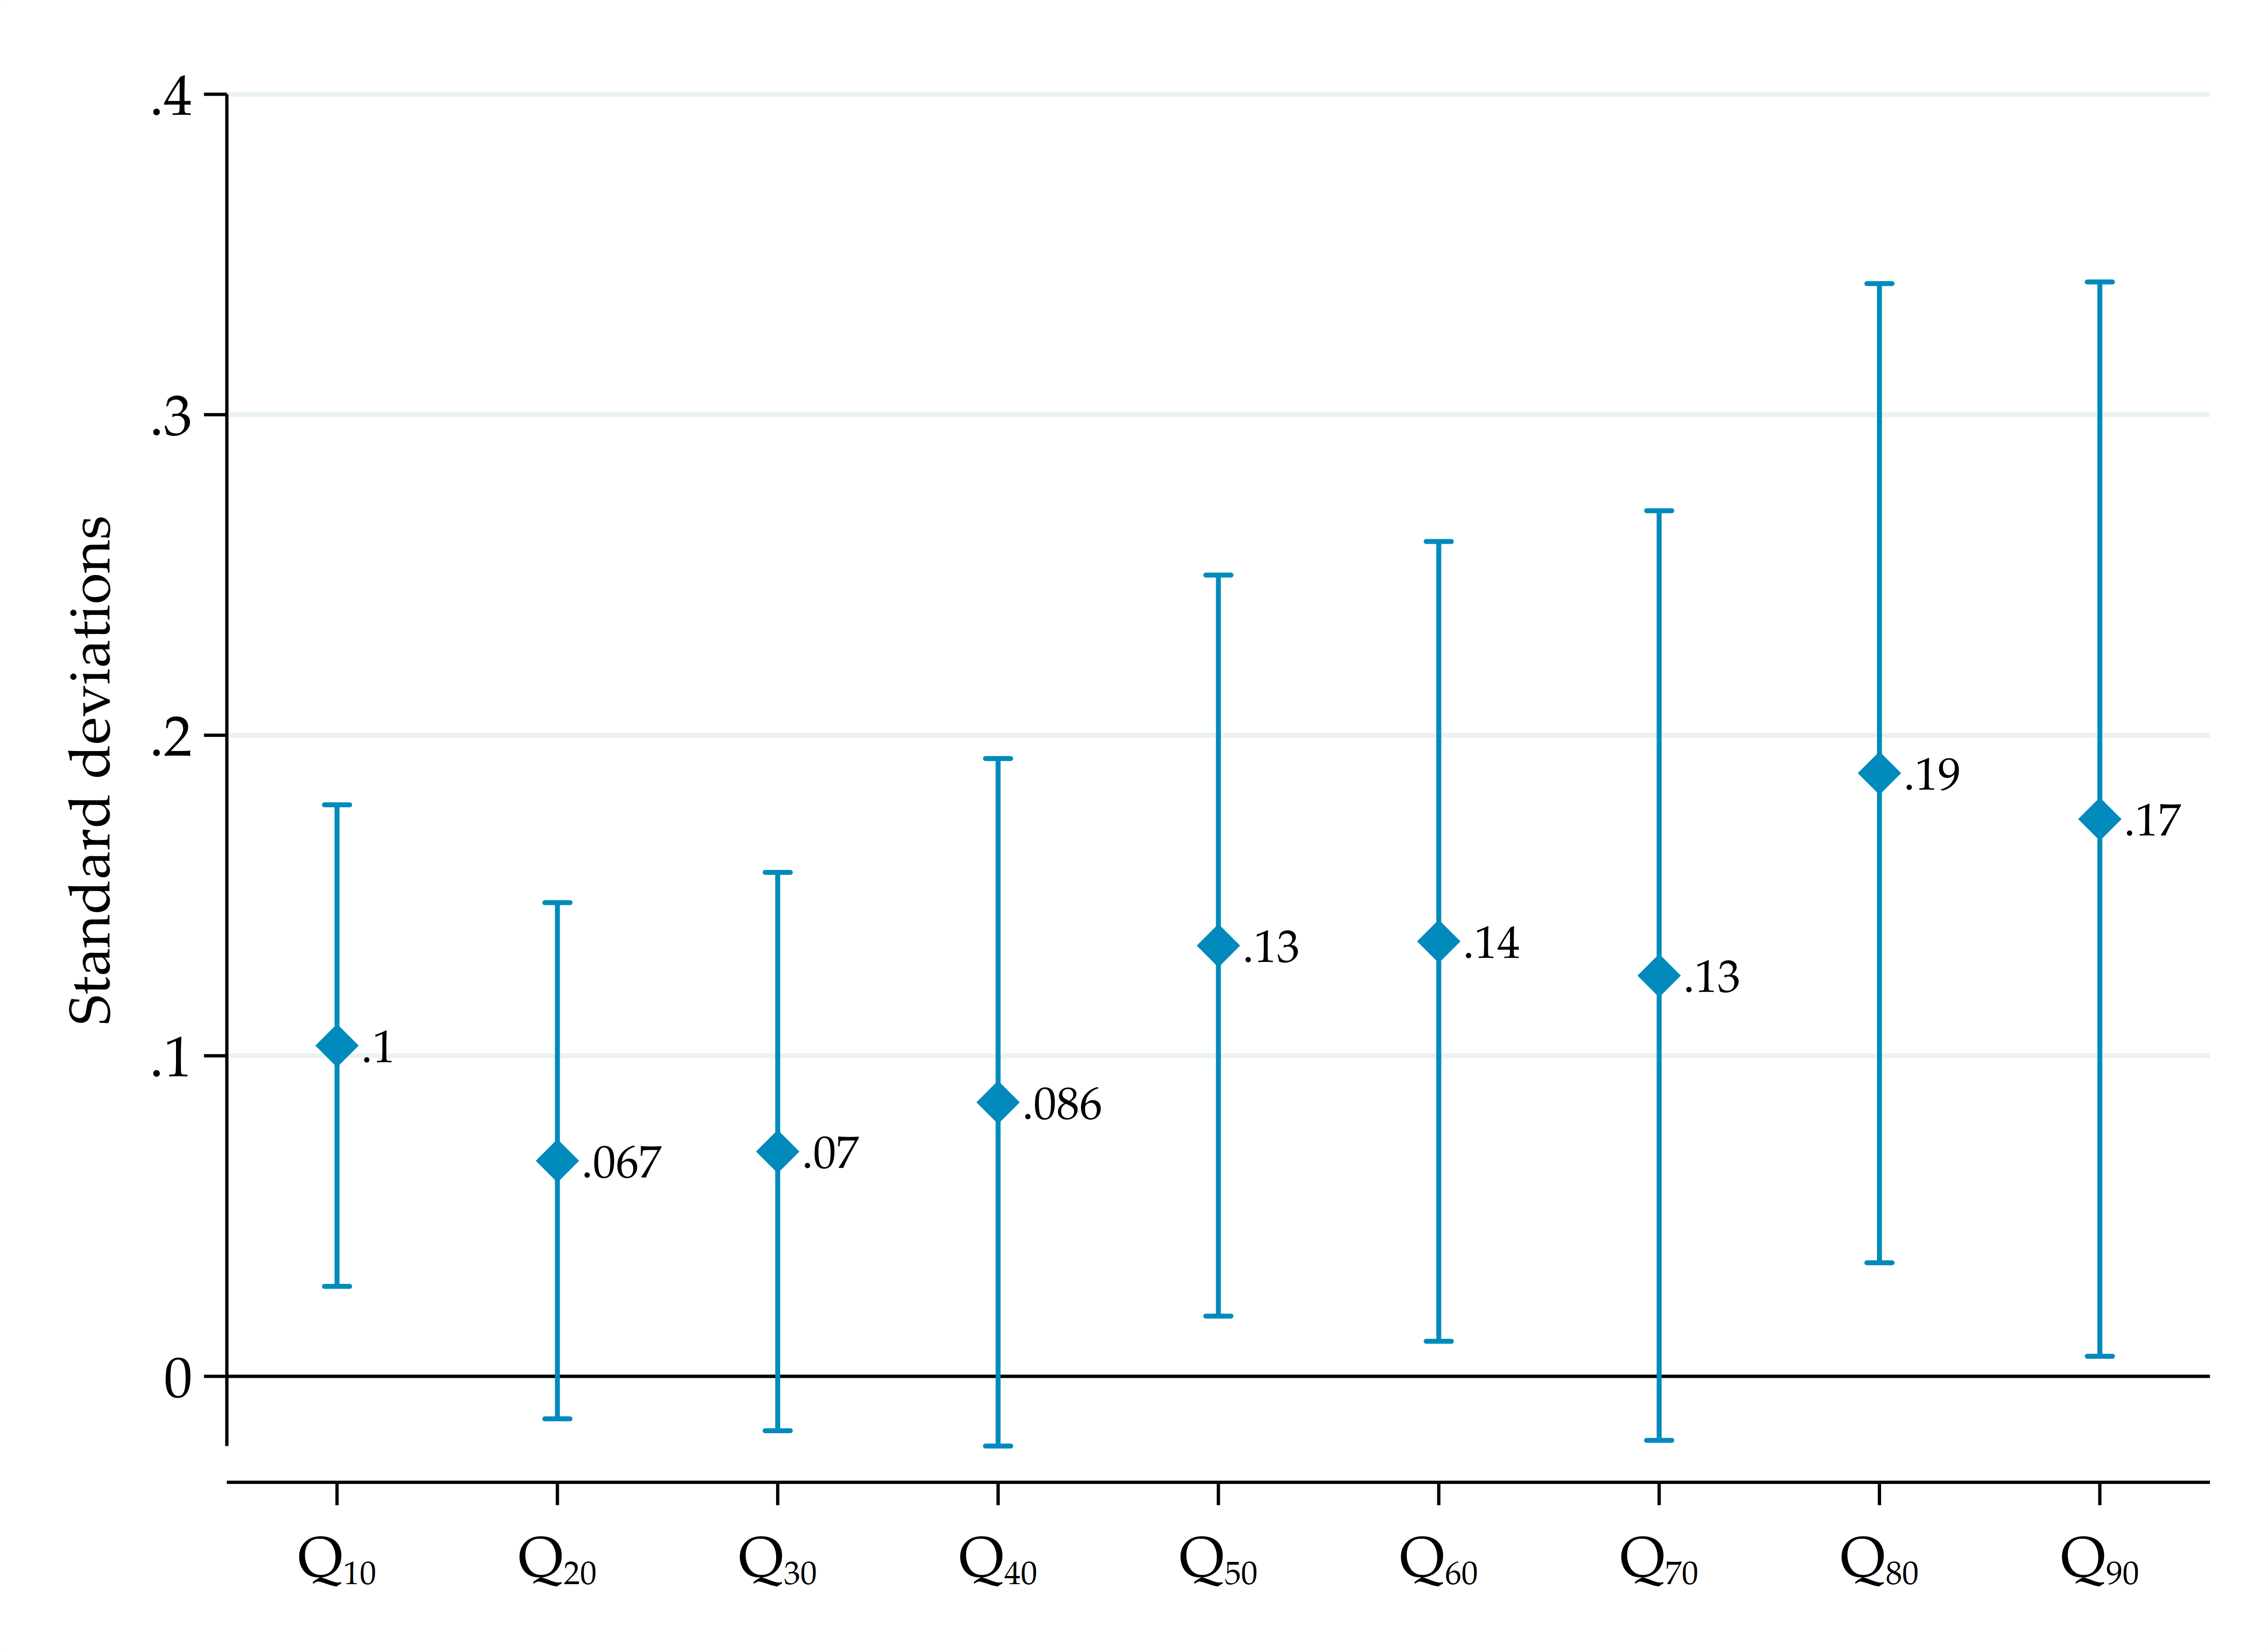
\includegraphics[width=8cm]{DataWork/Output/Figures/figC1d-qreg_CN_grade6}
		\end{subfigure}
		
		\vspace{1em}
		
		\justifying
		\noindent
		\small{\textit{Notes:} Point estimates of quantile regressions with strata (i.e., region and grade) fixed effects and standard errors clustered at the school level. Confidence intervals are 90\%. Quantile treatment effects are expressed in terms of standard deviations from the control group.}
	\end{figure}
	\vfill
	
	\null
	\vfill
	\begin{table}[!ht]
		\caption{Impact on Student Learning -- Controlling for Students' Characteristics}
		\centering
		\label{tab:test_studentlevel_ctrl}
		\begin{adjustbox}{max width=\textwidth}
			\begin{tabular}{lcccccc} \hline \hline
				&(1)     &(2)  &(3)        &(4)          &(5)                                                  \\               
&Average &Math &Portuguese &Human    &Natural                                          \\       
&        &            &                &Sciences &Sciences                                     \\ \hline
\multicolumn{6}{c}{\textbf{All schools}}                                                       \\ \hline
           Treatment   &       0.025         &       0.048         &       0.011         &      -0.010         &       0.047         \\              &     (0.045)         &     (0.053)         &     (0.055)         &     (0.042)         &     (0.042)         \\    Number of observations&        7501         &        6735         &        6738         &        6473         &        6468         \\  Number of clusters&         247         &         246         &         246         &         246         &         246         \\  Mean dep.\ var.\ control group&     183.110         &     172.557         &     191.239         &     183.849         &     183.181         \\  SD dep.\ var.\ control group&      41.531         &      47.868         &      53.273         &      49.299         &      42.794         \\  \hline
\multicolumn{6}{c}{\textbf{5th  grade -- Primary schools}}             \\ \hline
           Treatment   &      -0.083         &      -0.082         &      -0.134\sym{*}  &      -0.076         &      -0.074         \\              &     (0.073)         &     (0.087)         &     (0.073)         &     (0.078)         &     (0.078)         \\    Number of observations&        1865         &        1719         &        1721         &        1748         &        1746         \\  Number of clusters&          89         &          89         &          89         &          89         &          89         \\  Mean dep.\ var.\ control group&     161.031         &     161.372         &     178.781         &     156.159         &     151.470         \\  SD dep.\ var.\ control group&      35.929         &      44.061         &      58.953         &      36.943         &      28.855         \\  \hline
\multicolumn{6}{c}{\textbf{6th  grade -- Lower secondary schools}} \\ \hline
           Treatment   &       0.136\sym{**} &       0.180\sym{**} &       0.152\sym{*}  &       0.084         &       0.118\sym{*}  \\              &     (0.061)         &     (0.069)         &     (0.080)         &     (0.059)         &     (0.063)         \\    Number of observations&        3002         &        2679         &        2680         &        2749         &        2748         \\  Number of clusters&          97         &          96         &          96         &          97         &          97         \\  Mean dep.\ var.\ control group&     163.481         &     152.810         &     172.690         &     161.140         &     171.146         \\  SD dep.\ var.\ control group&      32.253         &      43.631         &      47.617         &      36.038         &      35.516         \\  \hline
\multicolumn{6}{c}{\textbf{10th grade -- Upper secondary schools}} \\ \hline
           Treatment   &      -0.042         &      -0.033         &      -0.063         &      -0.091         &       0.020         \\              &     (0.076)         &     (0.093)         &     (0.100)         &     (0.067)         &     (0.058)         \\    Number of observations&        2634         &        2337         &        2337         &        1976         &        1974         \\  Number of clusters&          61         &          61         &          61         &          60         &          60         \\  Mean dep.\ var.\ control group&     218.601         &     201.511         &     219.796         &     236.099         &     225.179         \\  SD dep.\ var.\ control group&      27.325         &      40.126         &      41.401         &      27.222         &      24.689         \\  \hline \hline

				\multicolumn{6}{@{}p{0.91\textwidth}}{\footnotesize \textit{Notes}: \sym{*}Significant at 10\%. \sym{**}Significant at 5\%. \sym{***}Significant at 1\%. Unit of observation: student. All regressions are OLS with strata fixed effects and control for students' characteristics, such as age, gender and race dummies (white, indigenous, black, or \textit{pardo}), whether they receive \textit{Bolsa Familia}, and  whether they use school transportation. Standard errors clustered at the school level in parentheses.}
			\end{tabular}
		\end{adjustbox}
	\end{table}
	\vfill
	
	\begin{table}[!ht]
		\caption{Impact on Student Learning -- Blocked Difference-in-Means}
		\label{tab:test_studentlevel_DIM}
		\centering
		\begin{adjustbox}{max width=\textwidth}
			\begin{tabular}{lcccccc} \hline \hline
				&(1)     &(2)  &(3)        &(4)          &(5)                                                  \\               
&Average &Math &Portuguese &Human    &Natural                                          \\       
&        &     &                       &Sciences &Sciences                                     \\ \hline
\multicolumn{6}{c}{\textbf{All schools}}                                               \\ \hline
           Treatment   &      -0.010         &      -0.018         &      -0.022         &      -0.010         &       0.024         \\              &     (0.058)         &     (0.065)         &     (0.078)         &     (0.046)         &     (0.041)         \\    Number of observations&       12760         &       11366         &       11365         &       10885         &       10879         \\  Number of clusters&         264         &         264         &         264         &         264         &         264         \\  Mean dep.\ var.\ control group&     184.052         &     172.693         &     190.234         &     186.477         &     185.329         \\  SD dep.\ var.\ control group&      41.081         &      46.528         &      52.637         &      49.517         &      42.864         \\  \hline
\multicolumn{6}{c}{\textbf{5th  grade -- Primary schools}}             \\ \hline
           Treatment   &      -0.123         &      -0.124         &      -0.134         &      -0.121         &      -0.130         \\              &     (0.097)         &     (0.108)         &     (0.100)         &     (0.098)         &     (0.090)         \\    Number of observations&        3179         &        2885         &        2885         &        2977         &        2978         \\  Number of clusters&          92         &          92         &          92         &          92         &          92         \\  Mean dep.\ var.\ control group&     157.452         &     157.540         &     173.368         &     154.288         &     149.499         \\  SD dep.\ var.\ control group&      36.022         &      43.798         &      60.456         &      37.359         &      28.700         \\  \hline
\multicolumn{6}{c}{\textbf{6th  grade -- Lower secondary schools}} \\ \hline
           Treatment   &       0.140\sym{**} &       0.154\sym{*}  &       0.163\sym{*}  &       0.095         &       0.124\sym{*}  \\              &     (0.069)         &     (0.081)         &     (0.083)         &     (0.061)         &     (0.066)         \\    Number of observations&        4511         &        4014         &        4013         &        4134         &        4131         \\  Number of clusters&          99         &          99         &          99         &          99         &          99         \\  Mean dep.\ var.\ control group&     162.845         &     151.930         &     172.451         &     160.075         &     170.685         \\  SD dep.\ var.\ control group&      31.523         &      42.024         &      47.502         &      35.775         &      35.164         \\  \hline
\multicolumn{6}{c}{\textbf{10th grade -- Upper secondary schools}} \\ \hline
           Treatment   &      -0.061         &      -0.084         &      -0.094         &      -0.043         &       0.022         \\              &     (0.092)         &     (0.102)         &     (0.133)         &     (0.075)         &     (0.059)         \\    Number of observations&        5070         &        4467         &        4467         &        3774         &        3770         \\  Number of clusters&          73         &          73         &          73         &          73         &          73         \\  Mean dep.\ var.\ control group&     215.446         &     198.009         &     214.086         &     233.701         &     223.680         \\  SD dep.\ var.\ control group&      26.923         &      38.838         &      41.371         &      26.369         &      23.650         \\  \hline                                                                                                               \hline

				\multicolumn{6}{@{}p{0.9\textwidth}}{\footnotesize \textit{Notes}: \sym{*}Significant at 10\%. \sym{**}Significant at 5\%. \sym{***}Significant at 1\%. Unit of observation: student. Coefficients are sample-weighted average treatment effects of the within-block difference-in-means (Blocked DIM). Standard errors clustered at the school level in parentheses.}
			\end{tabular}
		\end{adjustbox}
	\end{table}
	
	\begin{table}[ht!]
		\caption{Impact on Student Learning -- Interaction-Weighted Estimator (IWE)}
		\centering
		\label{tab:test_studentlevel_IWE}
		\begin{adjustbox}{max width=\textwidth}
			\begin{tabular}{lcccccc} \hline \hline
				&(1)     &(2)  &(3)        &(4)          &(5)                                                  \\               
&Average &Math &Portuguese &Human    &Natural                                          \\       
&        &     &                       &Sciences &Sciences                                     \\ \hline
\multicolumn{6}{c}{\textbf{5th  grade -- Primary schools}}             \\ \hline
          Treatment   &      -0.064         &      -0.064         &      -0.088         &      -0.067         &      -0.071         \\              &     (0.084)         &     (0.094)         &     (0.088)         &     (0.084)         &     (0.081)         \\    Percentage difference between IWE and OLS&      -4.617         &      -4.112         &      -2.815         &      -4.536         &      -4.150         \\  P-value for joint test of equality between IWE and OLS&       0.107         &       0.064         &       0.146         &       0.103         &       0.038         \\  P-value for joint Wald Test for interactions&       0.556         &       0.557         &       0.655         &       0.547         &       0.401         \\  \hline
\multicolumn{6}{c}{\textbf{6th  grade -- Lower secondary schools}} \\ \hline
          Treatment   &       0.145\sym{**} &       0.177\sym{**} &       0.157\sym{**} &       0.102\sym{*}  &       0.121\sym{**} \\              &     (0.061)         &     (0.072)         &     (0.073)         &     (0.054)         &     (0.062)         \\    Percentage difference between IWE and OLS&      -0.679         &      -0.101         &      -0.788         &      -0.577         &      -1.095         \\  P-value for joint test of equality between IWE and OLS&       0.703         &       0.723         &       0.459         &       0.756         &       0.661         \\  P-value for joint Wald Test for interactions&       0.956         &       0.931         &       0.872         &       0.957         &       0.924         \\  \hline \hline

				\multicolumn{6}{@{}p{1.15\textwidth}}{\footnotesize \textit{Notes}: \sym{*}Significant at 10\%. \sym{**}Significant at 5\%. \sym{***}Significant at 1\%. Unit of observation: student. All estimates are IWE as in \citet{gibbons2018broken}. Standard errors clustered at the school level in parentheses. We only show results for 5\textsuperscript{th} and 6\textsuperscript{th} grade, because 10\textsuperscript{th} grade has one stratum with no variation in treatment assignment.}
			\end{tabular}
		\end{adjustbox}
	\end{table}
	
	\begin{table}[ht!]
		\caption{Impact on Student Learning -- Regression-Weighted Estimator (RWE)}
		\centering
		\label{tab:test_studentlevel_RWE}
		\begin{adjustbox}{max width=\textwidth}
			\begin{tabular}{lcccccc} \hline \hline
				&(1)     &(2)  &(3)        &(4)          &(5)                                                  \\               
&Average &Math &Portuguese &Human    &Natural                                          \\       
&        &     &                       &Sciences &Sciences                                     \\ \hline
\multicolumn{6}{c}{\textbf{All schools}}                                               \\ \hline
         Treatment   &       0.034         &       0.045         &       0.031         &       0.011         &       0.044         \\              &     (0.044)         &     (0.050)         &     (0.056)         &     (0.038)         &     (0.038)         \\    Percentage difference between RWE and OLS&       5.428         &       8.406         &       9.503         &     -11.609         &       0.050         \\  P-value for joint test of equality between RWE and OLS&       0.423         &       0.134         &       0.334         &       0.394         &       0.991         \\     \hline
\multicolumn{6}{c}{\textbf{5th  grade -- Primary schools}}             \\ \hline
         Treatment   &      -0.065         &      -0.065         &      -0.088         &      -0.067         &      -0.071         \\              &     (0.087)         &     (0.097)         &     (0.090)         &     (0.087)         &     (0.084)         \\    Percentage difference between RWE and OLS&      -4.334         &      -3.803         &      -2.605         &      -4.230         &      -3.891         \\  P-value for joint test of equality between RWE and OLS&       0.091         &       0.131         &       0.175         &       0.109         &       0.056         \\  \hline
\multicolumn{6}{c}{\textbf{6th  grade -- Lower secondary schools}} \\ \hline
         Treatment   &       0.145\sym{**} &       0.177\sym{**} &       0.157\sym{**} &       0.102\sym{*}  &       0.121\sym{**} \\              &     (0.061)         &     (0.073)         &     (0.075)         &     (0.054)         &     (0.062)         \\    Percentage difference between RWE and OLS&      -0.663         &      -0.107         &      -0.752         &      -0.569         &      -1.053         \\  P-value for joint test of equality between RWE and OLS&       0.345         &       0.790         &       0.165         &       0.518         &       0.262         \\  \hline
\multicolumn{6}{c}{\textbf{10th grade -- Upper secondary schools}} \\ \hline
         Treatment   &      -0.004         &      -0.004         &      -0.006         &      -0.029         &       0.051         \\              &     (0.076)         &     (0.086)         &     (0.109)         &     (0.061)         &     (0.053)         \\    Percentage difference between RWE and OLS&     -59.928         &     -74.784         &     -62.107         &      10.203         &       0.484         \\  P-value for joint test of equality between RWE and OLS&       0.256         &       0.063         &       0.195         &       0.557         &       0.962         \\  \hline                                                                                                               \hline

				\multicolumn{6}{@{}p{1.15\textwidth}}{\footnotesize \textit{Notes}: \sym{*}Significant at 10\%. \sym{**}Significant at 5\%. \sym{***}Significant at 1\%. Unit of observation: student. All estimates are RWE as in \citet{gibbons2018broken}. Standard errors clustered at the school level in parentheses.}
			\end{tabular}
		\end{adjustbox}
	\end{table}
	
	\begin{table}[ht!]
		\caption{Impact on Student Learning -- School Level Regressions}
		\label{tab:test_schoollevel}
		\centering
		\begin{adjustbox}{max width=\textwidth}
			\begin{tabular}{lcccccc} \hline \hline
				&(1)     &(2)  &(3)        &(4)          &(5)                                                  \\               
&Average &Math &Portuguese &Human    &Natural                                          \\       
&        &     &                       &Sciences &Sciences                                     \\ \hline
\multicolumn{6}{c}{\textbf{All schools}}                                               \\ \hline
          Treatment   &       0.007         &       0.012         &      -0.007         &      -0.012         &       0.023         \\              &     (0.047)         &     (0.053)         &     (0.056)         &     (0.045)         &     (0.043)         \\    Number of observations&         263         &         263         &         263         &         263         &         263         \\  Mean dep.\ var.\ control group&     174.729         &     165.605         &     182.673         &     177.650         &     177.633         \\  SD dep.\ var.\ control group&      28.554         &      25.473         &      27.435         &      36.662         &      32.436         \\     \hline
\multicolumn{6}{c}{\textbf{5th  grade -- Primary schools}}             \\ \hline
          Treatment   &      -0.073         &      -0.070         &      -0.095         &      -0.070         &      -0.068         \\              &     (0.088)         &     (0.098)         &     (0.093)         &     (0.088)         &     (0.086)         \\    Number of observations&          92         &          92         &          92         &          92         &          92         \\  Mean dep.\ var.\ control group&     155.323         &     154.385         &     169.916         &     152.488         &     147.769         \\  SD dep.\ var.\ control group&      17.048         &      19.485         &      25.530         &      15.121         &      12.779         \\  \hline
\multicolumn{6}{c}{\textbf{6th  grade -- Lower secondary schools}} \\ \hline
          Treatment   &       0.152\sym{**} &       0.177\sym{**} &       0.170\sym{**} &       0.112\sym{**} &       0.135\sym{**} \\              &     (0.063)         &     (0.076)         &     (0.079)         &     (0.056)         &     (0.064)         \\    Number of observations&          99         &          99         &          99         &          99         &          99         \\  Mean dep.\ var.\ control group&     162.781         &     152.310         &     171.844         &     159.607         &     170.514         \\  SD dep.\ var.\ control group&      12.395         &      14.902         &      17.670         &       9.929         &      12.829         \\  \hline
\multicolumn{6}{c}{\textbf{10th grade -- Upper secondary schools}} \\ \hline
          Treatment   &      -0.019         &      -0.027         &      -0.050         &      -0.046         &       0.043         \\              &     (0.076)         &     (0.086)         &     (0.108)         &     (0.065)         &     (0.053)         \\    Number of observations&          72         &          72         &          72         &          72         &          72         \\  Mean dep.\ var.\ control group&     215.228         &     197.963         &     213.461         &     233.734         &     224.181         \\  SD dep.\ var.\ control group&       8.703         &      11.379         &      13.835         &       7.299         &       5.995         \\  \hline                                                                                                               \hline

				\multicolumn{6}{@{}p{0.92\textwidth}}{\footnotesize \textit{Notes}: \sym{*}Significant at 10\%. \sym{**}Significant at 5\%. \sym{***}Significant at 1\%. Unit of observation: school. All regressions are OLS with strata (i.e., region and grade) fixed effects and analytic weights for number of students enrolled in the grade of interest. Robust standard errors in parentheses. The coefficient are expressed in terms of standard deviations from the control group, while mean and standard deviation of the dependent variable refer to the raw values in the control group.}
			\end{tabular}
		\end{adjustbox}
	\end{table}
	
	\begin{table}[ht!]
		\caption{Impact on Student Learning -- Standardized Test Scores Rescaled to SAEB}
		\label{tab:test_rescaled_studentlevel}
		\centering
		\begin{adjustbox}{max width=\textwidth}
			\begin{tabular}{lccccc} \hline \hline &(1) &(2) &(3) &(4)  &(5)  \\
&5th &6th &9th &10th &12th \\ \cmidrule(lr){2-2} \cmidrule(lr){3-4} \cmidrule(lr){5-6}
\multicolumn{6}{c}{\textbf{Math}}       \\ \hline
           Treatment   &      -0.081         &       0.153\sym{**} &       0.117         &      -0.002         &      -0.078         \\              &     (0.094)         &     (0.073)         &     (0.092)         &     (0.085)         &     (0.114)         \\    Number of observations&        3065         &        4226         &        2118         &        4744         &        3257         \\  Number of clusters&          96         &         104         &          93         &          78         &          77         \\  Mean dep. var. control group&     164.623         &     173.851         &     211.814         &     220.419         &     234.287         \\  SD dep. var. control group&      46.278         &      44.655         &      45.455         &      37.330         &      42.500         \\  \hline
\multicolumn{6}{c}{\textbf{Portuguese}} \\ \hline
           Treatment   &      -0.092         &       0.133\sym{*}  &       0.115         &      -0.014         &      -0.029         \\              &     (0.087)         &     (0.076)         &     (0.085)         &     (0.107)         &     (0.112)         \\    Number of observations&        3065         &        4225         &        2119         &        4744         &        3260         \\  Number of clusters&          96         &         104         &          93         &          78         &          77         \\  Mean dep. var. control group&     178.878         &     179.134         &     218.859         &     223.413         &     231.668         \\  SD dep. var. control group&      64.768         &      51.032         &      49.923         &      44.412         &      46.331         \\  \hline \hline
 \multicolumn{6}{@{}p{0.87\textwidth}}{\footnotesize \textit{Notes}: \sym{*}Significant at 10\%. \sym{**}Significant at 5\%. \sym{***}Significant at 1\%. Unit of observation: student. All regressions are OLS with strata (i.e., region and grade) fixed effects. Standard errors clustered at the school level.}
			\end{tabular}
		\end{adjustbox}
	\end{table}
	
	% Spillover in other grades in the same year
	\begin{table}[ht!]
		\caption{Impact on Student Progression Rates in 6\textsuperscript{th} Grade Treated Schools -- Spillover to Other Grades}
		\label{tab:promotion_other_grades}
		\centering
		\begin{adjustbox}{max width=\textwidth}
			\begin{tabular}{lcccccccc} \hline \hline
				&\multicolumn{4}{c}{\textit{Grade level}} & \multicolumn{4}{c}{\textit{Student level}} \\
 \cmidrule(lr){2-5}                                             \cmidrule(lr){6-9} 
&(1) &(2) &(3) &(4) &(5) &(6) &(7) &(8) \\       
&6th &7th &8th &9th &6th &7th &8th &9th \\ \hline
&\multicolumn{8}{c}{\textbf{Passing}}   \\ \hline
           Treatment   &        8.46\sym{**} &       -0.16         &       -1.60         &       -4.62         &        7.00\sym{**} &        1.41         &       -0.46         &        0.95         \\              &      (3.30)         &      (2.93)         &      (2.64)         &      (3.23)         &      (3.10)         &      (3.18)         &      (2.88)         &      (3.61)         \\    Number of observations&         104         &         103         &          99         &          93         &        5490         &        4465         &        3294         &        2883         \\  Number of clusters&                     &                     &                     &                     &         104         &         103         &          99         &          93         \\  Mean dep.\ var.\ control group&       63.56         &       72.63         &       86.08         &       86.24         &       58.73         &       66.93         &       80.92         &       77.79         \\  SD dep.\ var.\ control group&       17.05         &       13.46         &       12.32         &       10.94         &       49.24         &       47.06         &       39.30         &       41.58         \\  \hline
&\multicolumn{8}{c}{\textbf{Dropout}}   \\ \hline
           Treatment   &       -1.61         &       -0.31         &        0.05         &        4.15         &       -4.35\sym{**} &       -2.88         &       -1.32         &       -3.78\sym{*}  \\              &      (1.27)         &      (1.38)         &      (1.42)         &      (2.76)         &      (1.82)         &      (1.78)         &      (1.75)         &      (2.25)         \\    Number of observations&         104         &         103         &          99         &          93         &        5494         &        4473         &        3303         &        2889         \\  Number of clusters&                     &                     &                     &                     &         104         &         103         &          99         &          93         \\  Mean dep.\ var.\ control group&        6.84         &        5.67         &        4.73         &        5.69         &       13.55         &       13.57         &       11.37         &       15.10         \\  SD dep.\ var.\ control group&        7.15         &        6.57         &        7.16         &        7.23         &       34.23         &       34.25         &       31.75         &       35.82         \\   \hline
&\multicolumn{8}{c}{\textbf{Retention}} \\ \hline
           Treatment   &       -6.85\sym{**} &        0.48         &        1.55         &        0.47         &       -2.65         &        1.46         &        1.84         &        2.84         \\              &      (2.91)         &      (2.89)         &      (2.13)         &      (2.08)         &      (2.81)         &      (2.74)         &      (1.74)         &      (2.08)         \\    Number of observations&         104         &         103         &          99         &          93         &        5490         &        4465         &        3294         &        2883         \\  Number of clusters&                     &                     &                     &                     &         104         &         103         &          99         &          93         \\  Mean dep.\ var.\ control group&       29.59         &       21.70         &        9.19         &        8.07         &       27.72         &       19.48         &        7.65         &        7.08         \\  SD dep.\ var.\ control group&       14.91         &       12.37         &       10.02         &        9.51         &       44.77         &       39.61         &       26.60         &       25.66         \\  \hline \hline

				\multicolumn{9}{@{}p{1.05\textwidth}}{\footnotesize \textit{Notes}: \sym{*}Significant at 10\%. \sym{**}Significant at 5\%. \sym{***}Significant at 1\%. School-level data are from \textit{Sistema Integrado de Gestão da Educação} (SIGEduc) and student-level data are from Rio Grande do Norte census. Unit of observation: school and student. Sample: schools treated at 6\textsuperscript{th} grade. All regressions are OLS with strata (i.e., region) fixed effects. Robust standard errors for school-level regressions and standard errors clustered at the school level for student-level regressions in parentheses.}
			\end{tabular}
		\end{adjustbox}
	\end{table}
	
	\begin{table}[ht!]
		\caption{Impact on Student Progression Rates in 6\textsuperscript{th} Grade Treated Schools by Teacher Turnover at Baseline -- Spillover to Other Grades}
		\label{tab:het_spillover_other_grades}
		\centering
		\begin{adjustbox}{totalheight=\textheight-2\baselineskip}
			\begin{tabular}{lccc} \hline \hline
				&(1) &(2) &(3)                                                                                                         \\             
&7th &8th &9th                                                                                                         \\ \hline  
\multicolumn{4}{c}{\textit{Probability of student passing}}            \\ \hline  
                    Treatment   &       0.052         &      -0.046         &       0.006         \\              &     (0.046)         &     (0.030)         &     (0.043)         \\    Treatment $\times$ High teacher turnover at baseline&      -0.055         &       0.070         &       0.014         \\              &     (0.061)         &     (0.054)         &     (0.069)         \\    High teacher turnover at baseline&      -0.051         &      -0.092\sym{**} &      -0.045         \\              &     (0.041)         &     (0.038)         &     (0.034)         \\    \addlinespace[0.5em] Constant&       0.695\sym{***}&       0.862\sym{***}&       0.791\sym{***}\\              &     (0.029)         &     (0.019)         &     (0.019)         \\    \addlinespace[0.75em] Number of observations&        4299         &        3205         &        2828         \\  Number of clusters&          97         &          95         &          90         \\  \addlinespace[0.75em] \multicolumn{4}{l}{\textit{Total effect:} Treatment $+$ Treatment $\times$ High teacher turnover at baseline} \\ \hspace{10pt} $\sum \hat{\beta}$&      -0.003         &       0.024         &       0.020         \\  \hspace{10pt} P-value&       0.948         &       0.603         &       0.721         \\  \hline
\multicolumn{4}{c}{\textit{Probability of student dropping out}}   \\ \hline  
                    Treatment   &      -0.056\sym{***}&      -0.014         &      -0.034         \\              &     (0.018)         &     (0.019)         &     (0.031)         \\    Treatment $\times$ High teacher turnover at baseline&       0.030         &       0.000         &      -0.007         \\              &     (0.030)         &     (0.033)         &     (0.044)         \\    High teacher turnover at baseline&       0.024         &       0.039         &      -0.003         \\              &     (0.024)         &     (0.027)         &     (0.025)         \\    \addlinespace[0.5em] Constant&       0.126\sym{***}&       0.093\sym{***}&       0.159\sym{***}\\              &     (0.017)         &     (0.015)         &     (0.018)         \\    \addlinespace[0.75em] Number of observations&        4307         &        3214         &        2833         \\  Number of clusters&          97         &          95         &          90         \\  \addlinespace[0.75em] \multicolumn{4}{l}{\textit{Total effect:} Treatment $+$ Treatment $\times$ High teacher turnover at baseline} \\ \hspace{10pt} $\sum \hat{\beta}$&      -0.027         &      -0.014         &      -0.041         \\  \hspace{10pt} P-value&       0.289         &       0.615         &       0.205         \\   \hline
\multicolumn{4}{c}{\textit{Probability of student being retained}} \\ \hline  
                    Treatment   &       0.004         &       0.062\sym{***}&       0.027         \\              &     (0.045)         &     (0.022)         &     (0.021)         \\    Treatment $\times$ High teacher turnover at baseline&       0.026         &      -0.071\sym{**} &      -0.006         \\              &     (0.055)         &     (0.033)         &     (0.038)         \\    High teacher turnover at baseline&       0.026         &       0.054\sym{**} &       0.047\sym{**} \\              &     (0.034)         &     (0.023)         &     (0.021)         \\    \addlinespace[0.5em] Constant&       0.179\sym{***}&       0.044\sym{***}&       0.050\sym{***}\\              &     (0.027)         &     (0.015)         &     (0.010)         \\    \addlinespace[0.75em] Number of observations&        4299         &        3205         &        2828         \\  Number of clusters&          97         &          95         &          90         \\  \addlinespace[0.75em] \multicolumn{4}{l}{\textit{Total effect:} Treatment $+$ Treatment $\times$ High teacher turnover at baseline} \\ \hspace{10pt} $\sum \hat{\beta}$&       0.030         &      -0.010         &       0.022         \\  \hspace{10pt} P-value&       0.372         &       0.693         &       0.504         \\  \hline                                                                                                     \hline  
                                                                                                                                       \\ [-1.8ex]
				\multicolumn{4}{@{}p{0.85\textwidth}}{\footnotesize \textit{Notes}: \sym{*}Significant at 10\%. \sym{**}Significant at 5\%. \sym{***}Significant at 1\%. Student and teacher data are from Rio Grande do Norte censuses. Unit of observation: student. Sample: schools treated at 6\textsuperscript{th} grade. $\sum \hat{\beta}$ is the sum of the treatment effect with the interaction variable coefficient. The p-value refers to the null hypothesis $\sum \hat{\beta} = 0$. All regressions are OLS with strata (i.e., region) fixed effects. the coefficients on progression are expressed in terms of percentage points. Standard errors clustered at the school level in parentheses.}
			\end{tabular}
		\end{adjustbox}
	\end{table}

	\begin{table}[ht!]
		\caption{Impact on Socio-Emotional Skills -- Controlling for Students' Characteristics}
		\centering
		\label{tab:socio_studentlevel_ctrl}
		\begin{adjustbox}{max width=\textwidth}
			\begin{tabular}{lccccc} \hline \hline
				&(1)                   &(2)                       &(3)          &(4)             &(5)          \\               
&Agreeableness &Conscientiousness &Extroversion &Neuroticism &Openness \\ \hline
\multicolumn{6}{c}{\textbf{All schools}}                                                               \\ \hline
           Treatment   &       0.059         &       0.118\sym{*}  &       0.099\sym{*}  &       0.098         &       0.042         \\              &     (0.063)         &     (0.061)         &     (0.059)         &     (0.061)         &     (0.061)         \\    Number of observations&        2141         &        2141         &        2141         &        2141         &        2141         \\  Number of clusters&         213         &         213         &         213         &         213         &         213         \\  Mean dep. var. control group&       4.419         &       4.347         &       4.206         &       3.993         &       4.122         \\  SD dep. var. control group&       0.983         &       1.060         &       0.788         &       0.741         &       0.964         \\  \hline
\multicolumn{6}{c}{\textbf{5th  grade -- Primary schools}}                     \\ \hline
           Treatment   &      -0.058         &      -0.001         &      -0.017         &      -0.023         &      -0.102         \\              &     (0.087)         &     (0.096)         &     (0.092)         &     (0.083)         &     (0.091)         \\    Number of observations&         778         &         778         &         778         &         778         &         778         \\  Number of clusters&          82         &          82         &          82         &          82         &          82         \\  Mean dep. var. control group&       4.552         &       4.436         &       4.347         &       4.099         &       4.262         \\  SD dep. var. control group&       1.034         &       1.124         &       0.834         &       0.754         &       0.987         \\  \hline
\multicolumn{6}{c}{\textbf{6th  grade -- Lower secondary schools}}     \\ \hline
           Treatment   &       0.076         &       0.139         &       0.163         &       0.145         &       0.070         \\              &     (0.119)         &     (0.109)         &     (0.104)         &     (0.119)         &     (0.108)         \\    Number of observations&         796         &         796         &         796         &         796         &         796         \\  Number of clusters&          82         &          82         &          82         &          82         &          82         \\  Mean dep. var. control group&       4.356         &       4.281         &       4.125         &       3.917         &       3.962         \\  SD dep. var. control group&       1.077         &       1.152         &       0.860         &       0.752         &       1.054         \\  \hline
\multicolumn{6}{c}{\textbf{10th grade -- Upper secondary schools}}     \\ \hline
           Treatment   &       0.182         &       0.235\sym{**} &       0.148\sym{*}  &       0.187\sym{*}  &       0.194\sym{*}  \\              &     (0.110)         &     (0.097)         &     (0.086)         &     (0.101)         &     (0.105)         \\    Number of observations&         567         &         567         &         567         &         567         &         567         \\  Number of clusters&          49         &          49         &          49         &          49         &          49         \\  Mean dep. var. control group&       4.324         &       4.325         &       4.130         &       3.965         &       4.180         \\  SD dep. var. control group&       0.674         &       0.752         &       0.519         &       0.687         &       0.700         \\  \hline                                                                                                                       \hline

				\multicolumn{6}{@{}p{1.175\textwidth}}{\footnotesize \textit{Notes}: \sym{*}Significant at 10\%. \sym{**}Significant at 5\%. \sym{***}Significant at 1\%. Unit of observation: student. All regressions are OLS with strata (i.e., region and grade) fixed effects and control for students' characteristics, such as age, gender and race dummies (white, indigenous, black, or \textit{pardo}), whether they receive \textit{Bolsa Familia}, and whether they use school transportation. Standard errors clustered at the school level in parentheses.}
			\end{tabular}
		\end{adjustbox}
	\end{table}
	
	\begin{table}[ht!]
		\caption{Impact on Socio-Emotional Skills -- Blocked Difference-in-Means}
		\label{tab:socio_studentlevel_DIM}
		\centering
		\begin{adjustbox}{max width=\textwidth}
			\begin{tabular}{lcccccc} \hline \hline
				&(1)                   &(2)                       &(3)          &(4)             &(5)          \\               
&Agreeableness &Conscientiousness &Extroversion &Neuroticism &Openness \\ \hline
\multicolumn{6}{c}{\textbf{All schools}}                                                       \\ \hline
           Treatment   &       0.013         &       0.085         &       0.107\sym{*}  &       0.013         &       0.019         \\              &     (0.059)         &     (0.061)         &     (0.063)         &     (0.050)         &     (0.059)         \\    Number of observations&        3560         &        3560         &        3560         &        3558         &        3560         \\  Number of clusters&         235         &         235         &         235         &         235         &         235         \\  Mean dep.\ var.\ control group&       4.413         &       4.331         &       4.199         &       4.007         &       4.105         \\  SD dep.\ var.\ control group&       0.975         &       1.053         &       0.777         &       0.738         &       0.970         \\  \hline
\multicolumn{6}{c}{\textbf{5th  grade -- Primary schools}}                     \\ \hline
           Treatment   &      -0.025         &       0.072         &       0.053         &       0.004         &      -0.085         \\              &     (0.102)         &     (0.104)         &     (0.112)         &     (0.079)         &     (0.103)         \\    Number of observations&        1296         &        1296         &        1296         &        1294         &        1296         \\  Number of clusters&          85         &          85         &          85         &          85         &          85         \\  Mean dep.\ var.\ control group&       4.468         &       4.359         &       4.287         &       4.040         &       4.193         \\  SD dep.\ var.\ control group&       1.049         &       1.108         &       0.851         &       0.738         &       0.997         \\  \hline
\multicolumn{6}{c}{\textbf{6th  grade -- Lower secondary schools}}     \\ \hline
           Treatment   &       0.068         &       0.170\sym{*}  &       0.203\sym{**} &       0.009         &       0.120         \\              &     (0.095)         &     (0.100)         &     (0.099)         &     (0.084)         &     (0.095)         \\    Number of observations&        1270         &        1270         &        1270         &        1270         &        1270         \\  Number of clusters&          87         &          87         &          87         &          87         &          87         \\  Mean dep.\ var.\ control group&       4.390         &       4.265         &       4.156         &       3.971         &       3.950         \\  SD dep.\ var.\ control group&       1.090         &       1.176         &       0.858         &       0.770         &       1.089         \\  \hline
\multicolumn{6}{c}{\textbf{10th grade -- Upper secondary schools}}     \\ \hline
           Treatment   &       0.011         &      -0.006         &       0.075         &       0.036         &       0.072         \\              &     (0.098)         &     (0.086)         &     (0.091)         &     (0.091)         &     (0.083)         \\    Number of observations&         994         &         994         &         994         &         994         &         994         \\  Number of clusters&          63         &          63         &          63         &          63         &          63         \\  Mean dep.\ var.\ control group&       4.378         &       4.387         &       4.152         &       4.017         &       4.212         \\  SD dep.\ var.\ control group&       0.663         &       0.761         &       0.514         &       0.692         &       0.701         \\  \hline                                                                                                                       \hline

				\multicolumn{6}{@{}p{1.17\textwidth}}{\footnotesize \textit{Notes}: \sym{*}Significant at 10\%. \sym{**}Significant at 5\%. \sym{***}Significant at 1\%. Unit of observation: student. Coefficients are sample-weighted average treatment effects of the within-block difference-in-means (Blocked DIM). Standard errors clustered at the school level in parentheses.}
			\end{tabular}
		\end{adjustbox}
	\end{table}
	
	\begin{table}[ht!]
		\caption{Impact on Socio-Emotional Skills -- Interaction-Weighted Estimator (IWE)}
		\centering
		\label{tab:socio_studentlevel_IWE}
		\begin{adjustbox}{max width=\textwidth}
			\begin{tabular}{lcccccc} \hline \hline
				&(1)                   &(2)                       &(3)          &(4)             &(5)          \\               
&Agreeableness &Conscientiousness &Extroversion &Neuroticism &Openness \\ \hline
\multicolumn{6}{c}{\textbf{All schools}}                                                               \\ \hline
          Treatment   &       0.046         &       0.113\sym{**} &       0.113\sym{**} &       0.036         &       0.055         \\              &     (0.054)         &     (0.052)         &     (0.053)         &     (0.046)         &     (0.052)         \\    Percentage difference between IWE and OLS&      -4.587         &      -1.692         &      -2.212         &      -1.581         &      -5.082         \\  P-value for joint test of equality between IWE and OLS&       0.221         &       0.002         &       0.101         &       0.211         &       0.059         \\  P-value for joint Wald Test for interactions&       0.462         &       0.122         &       0.483         &       0.680         &       0.303         \\  \hline
\multicolumn{6}{c}{\textbf{5th  grade  -- Primary schools}}                    \\ \hline
          Treatment   &       0.023         &       0.093         &       0.048         &      -0.020         &      -0.062         \\              &     (0.095)         &     (0.094)         &     (0.096)         &     (0.073)         &     (0.092)         \\    Percentage difference between IWE and OLS&      -0.984         &      -0.341         &      -1.650         &       2.051         &       1.703         \\  P-value for joint test of equality between IWE and OLS&       0.745         &       0.890         &       0.467         &       0.868         &       0.861         \\  P-value for joint Wald Test for interactions&       0.945         &       0.989         &       0.815         &       0.984         &       0.980         \\  \hline
\multicolumn{6}{c}{\textbf{6th  grade  -- Lower secondary schools}}    \\ \hline
          Treatment   &       0.078         &       0.173\sym{*}  &       0.206\sym{**} &       0.060         &       0.138         \\              &     (0.097)         &     (0.096)         &     (0.096)         &     (0.091)         &     (0.096)         \\    Percentage difference between IWE and OLS&      -0.020         &      -0.147         &      -0.561         &       2.750         &      -0.233         \\  P-value for joint test of equality between IWE and OLS&       0.211         &       0.487         &       0.377         &       0.621         &       0.308         \\  P-value for joint Wald Test for interactions&       0.517         &       0.795         &       0.703         &       0.886         &       0.625         \\  \hline
\multicolumn{6}{c}{\textbf{10th  grade -- Upper secondary schools}}    \\ \hline
          Treatment   &       0.035         &       0.063         &       0.080         &       0.079         &       0.103         \\              &     (0.083)         &     (0.068)         &     (0.074)         &     (0.070)         &     (0.071)         \\    Percentage difference between IWE and OLS&     -16.644         &      -7.669         &      -5.785         &      -3.637         &      -6.341         \\  P-value for joint test of equality between IWE and OLS&       0.051         &       0.000         &       0.075         &       0.019         &       0.007         \\  P-value for joint Wald Test for interactions&       0.223         &       0.007         &       0.384         &       0.172         &       0.134         \\  \hline                                                                                                                       \hline

				\multicolumn{6}{@{}p{1.42\textwidth}}{\footnotesize \textit{Notes}: \sym{*}Significant at 10\%. \sym{**}Significant at 5\%. \sym{***}Significant at 1\%. Unit of observation: student. All estimates are IWE as in \citet{gibbons2018broken}. Standard errors clustered at the school level in parentheses.}
			\end{tabular}
		\end{adjustbox}
	\end{table}
	
	\begin{table}[ht!]
		\caption{Impact on Socio-Emotional Skills -- Regression-Weighted Estimator (RWE)}
		\centering
		\label{tab:socio_studentlevel_RWE}
		\begin{adjustbox}{max width=\textwidth}
			\begin{tabular}{lcccccc} \hline \hline
				&(1)                   &(2)                       &(3)          &(4)             &(5)          \\               
&Agreeableness &Conscientiousness &Extroversion &Neuroticism &Openness \\ \hline
\multicolumn{6}{c}{\textbf{All schools}}                                                       \\ \hline
         Treatment   &       0.046         &       0.113\sym{**} &       0.114\sym{**} &       0.036         &       0.055         \\              &     (0.056)         &     (0.054)         &     (0.054)         &     (0.047)         &     (0.054)         \\    Percentage difference between RWE and OLS&      -4.761         &      -1.763         &      -2.109         &      -1.953         &      -5.274         \\  P-value for joint test of equality between RWE and OLS&       0.248         &       0.183         &       0.109         &       0.587         &       0.053         \\  \hline
\multicolumn{6}{c}{\textbf{5th  grade -- Primary schools}}                     \\ \hline
         Treatment   &       0.023         &       0.093         &       0.048         &      -0.020         &      -0.062         \\              &     (0.096)         &     (0.095)         &     (0.096)         &     (0.074)         &     (0.093)         \\    Percentage difference between RWE and OLS&      -1.707         &      -0.373         &      -1.363         &       1.391         &       1.820         \\  P-value for joint test of equality between RWE and OLS&       0.889         &       0.895         &       0.796         &       0.907         &       0.650         \\  \hline
\multicolumn{6}{c}{\textbf{6th  grade -- Lower secondary schools}}     \\ \hline
         Treatment   &       0.078         &       0.173\sym{*}  &       0.207\sym{**} &       0.060         &       0.138         \\              &     (0.099)         &     (0.098)         &     (0.097)         &     (0.092)         &     (0.098)         \\    Percentage difference between RWE and OLS&       0.026         &      -0.111         &      -0.505         &       2.322         &      -0.220         \\  P-value for joint test of equality between RWE and OLS&       0.992         &       0.925         &       0.636         &       0.546         &       0.874         \\  \hline
\multicolumn{6}{c}{\textbf{10th grade -- Upper secondary schools}}     \\ \hline
         Treatment   &       0.035         &       0.063         &       0.080         &       0.079         &       0.102         \\              &     (0.092)         &     (0.079)         &     (0.078)         &     (0.074)         &     (0.080)         \\    Percentage difference between RWE and OLS&     -16.960         &      -8.219         &      -5.698         &      -3.997         &      -6.596         \\  P-value for joint test of equality between RWE and OLS&       0.175         &       0.058         &       0.123         &       0.177         &       0.080         \\  \hline                                                                                                                       \hline

				\multicolumn{6}{@{}p{1.42\textwidth}}{\footnotesize \textit{Notes}: \sym{*}Significant at 10\%. \sym{**}Significant at 5\%. \sym{***}Significant at 1\%. Unit of observation: student. All estimates are RWE as in \citet{gibbons2018broken}. Standard errors clustered at the school level in parentheses.}
			\end{tabular}
		\end{adjustbox}
	\end{table}
	
	\begin{table}[ht!]
		\caption{Impact on Socio-Emotional Skills -- School Level Regressions}
		\label{tab:socio_schoollevel}
		\centering
		\begin{adjustbox}{max width=\textwidth}
			\begin{tabular}{lcccccc} \hline \hline
				&(1)                   &(2)                       &(3)          &(4)             &(5)          \\               
&Agreeableness &Conscientiousness &Extroversion &Neuroticism &Openness \\ \hline
\multicolumn{6}{c}{\textbf{All schools}}                                                       \\ \hline
          Treatment   &       0.075         &       0.142\sym{**} &       0.103         &       0.087         &       0.078         \\              &     (0.076)         &     (0.069)         &     (0.069)         &     (0.062)         &     (0.069)         \\    Number of observations&         235         &         235         &         235         &         235         &         235         \\  Mean dep.\ var.\ control group&       4.379         &       4.293         &       4.162         &       3.966         &       4.049         \\  SD dep.\ var.\ control group&       0.566         &       0.612         &       0.468         &       0.355         &       0.582         \\     \hline
\multicolumn{6}{c}{\textbf{5th  grade -- Primary schools}}                     \\ \hline
          Treatment   &       0.086         &       0.157         &       0.050         &       0.092         &      -0.010         \\              &     (0.125)         &     (0.120)         &     (0.118)         &     (0.102)         &     (0.121)         \\    Number of observations&          85         &          85         &          85         &          85         &          85         \\  Mean dep.\ var.\ control group&       4.435         &       4.323         &       4.258         &       3.984         &       4.162         \\  SD dep.\ var.\ control group&       0.689         &       0.651         &       0.484         &       0.347         &       0.562         \\  \hline
\multicolumn{6}{c}{\textbf{6th  grade -- Lower secondary schools}}     \\ \hline
          Treatment   &       0.098         &       0.204\sym{*}  &       0.274\sym{**} &       0.096         &       0.182         \\              &     (0.120)         &     (0.111)         &     (0.124)         &     (0.096)         &     (0.124)         \\    Number of observations&          87         &          87         &          87         &          87         &          87         \\  Mean dep.\ var.\ control group&       4.359         &       4.211         &       4.080         &       3.938         &       3.853         \\  SD dep.\ var.\ control group&       0.595         &       0.718         &       0.573         &       0.406         &       0.702         \\  \hline
\multicolumn{6}{c}{\textbf{10th grade -- Upper secondary schools}}     \\ \hline
          Treatment   &       0.039         &       0.064         &       0.022         &       0.071         &       0.107         \\              &     (0.145)         &     (0.122)         &     (0.109)         &     (0.124)         &     (0.106)         \\    Number of observations&          63         &          63         &          63         &          63         &          63         \\  Mean dep.\ var.\ control group&       4.330         &       4.372         &       4.149         &       3.984         &       4.182         \\  SD dep.\ var.\ control group&       0.262         &       0.315         &       0.161         &       0.285         &       0.258         \\  \hline \hline

				\multicolumn{6}{@{}p{1.175\textwidth}}{\footnotesize \textit{Notes}: \sym{*}Significant at 10\%. \sym{**}Significant at 5\%. \sym{***}Significant at 1\%. Unit of observation: school. All regressions are OLS with strata (i.e., region and grade) fixed effects and analytic weights for number of students enrolled in the grade of interest. Robust standard errors in parentheses. The coefficient are expressed in terms of standard deviations from the control group, while mean and standard deviation of the dependent variable refer to the raw values in the control group.}
			\end{tabular}
		\end{adjustbox}
	\end{table}
	
	\bibliography{references}
		
\end{document}